\section{Zielsetzung}
\label{sec:Ziel}
In diesem Versuch sollen Strömungen und ihre Eigenschaften mithilfe der Doppler-Sonographie untersucht
werden. Dabei lassen sich über Impuls-Echo-Verfahren Strömungsprofil- und Geschwindigkeit ermitteln. 

\section{Theorie}
\label{sec:Theorie}

Grundlage dieses Versuchs ist der sogenannte Doppler-Effekt. Dieser beschreibt eine Änderung der Frequenz 
bei Wellen, wenn sich Quelle und Empfänger relativ zueinander bewegen.\\
\noindent Zulaufende, bewegte Quelle und ruhender Beobachter, verschieben die Frequenz $\nu_0$ zu höheren Frequenzen $\nu_{kl}$.\\
\noindent Fortlaufende, bewegte Quelle und ruhender Beobachter, verschieben die Frequenz  $\nu_0$ zu tieferen Frequenzen  $\nu_{gr}$.\\
\noindent Die verschobenen Frequenzen lassen sich dann mit 

\begin{equation}
    \nu_{kl/gr} = \dfrac{\nu_0}{1\mp\dfrac{v}{c}}
    \label{eq:eins}
\end{equation}

\noindent bestimmen.\\
\noindent Falls nun die Quelle ruht und der Beobachter sich auf diese zubewegt, wird  $\nu_0$ zu höheren Frequenzen $\nu_h$ verschoben. 
Bei einem sich von der ruhenden Quelle entfernendem Beobachter, ließe sich eine Verschiebung zu tieferen Frequenzen  $\nu_n$ feststellen.\\
\noindent In diesem Fall wird 

\begin{equation}
    \nu_{h/n} = \nu_0(1\pm\dfrac{v}{c})
    \label{eq:zwei}
\end{equation}

\noindent zur Ermittlung der Frequenzen verwendet.\\ 
\noindet Das Prinzip dieses Verfahrens wird in der Medizin bei Messungen der Geschwindigkeit von Blutströmungen eingesetzt.
Es lässt sich in \autoref{fig:blut} betrachten.

\begin{figure}[H]
    \centering
    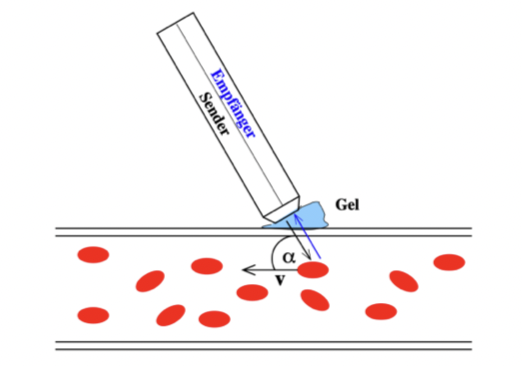
\includegraphics[width=\textwidth]{content/doppler.png}
    \caption{Schematische Anwendung des Doppler-Effekts bei Blutströmungen.\cite{anleitung}}
    \label{fig:blut}
\end{figure}

\noindent Wenn eine Ultraschallwelle auf ein bewegtes Objekt trifft, wird ihre Frequenz gemäß des Doppler-Effekts
verschoben. Diese Verschiebung ist durch

\begin{equation}
    \Delta\nu = \nu_0\dfrac{v}{c}(\cos{\alpha}+\cos{\beta})
    \label{eq:drei}
\end{equation}

\noindent definiert. Hierbei ist $v$ die Geschwindigkeit des bewegten Objekts (z.B. Blutkörperchen) und $c$ die Schallgeschwindigkeit.  
Zusätzlich ist die Verschiebung von den Winkeln $\alpha$ und $\beta$ abhängig. Diese befinden sich zwischen $v$ und der Wellennormalen.
In diesem Fall sind beide Winkel identisch, sodass sich 
\begin{equation}
    \Delta\nu = 2\nu_0\dfrac{v}{c}\cos{\alpha}
    \label{eq:vier}
\end{equation}

\noindent ergibt.\\
Der verwendete Ultraschall kann mit dem reziproken piezo-elektrischen Effekt erzeugt werden. 
Hierzu wird ein piezoelektrischer Kristall in ein elektrisches Wechselfeld gebracht, sodass 
dieser durch Schwingungen Ultraschall erzeugt. Dies geschieht, falls eine polare Achse des 
Kristalls in Richtung des E-Feldes zeigt. Zudem kann der Kristall durch externe Schallwellen
angeregt werden, sodass dieser auch als Schallempfänger fungieren kann. Eingesetzte Kristalle 
sind meist Quarze, die zwar einen schwachen piezoelektrischen Effekt haben, aber gleichbleibende 
physikalische Eigenschaften.

\section{Vorbereitung}
\label{sec:Vorbereitung}

Die Vorbereitungsaufgabe des Versuchs bestand darin, die Dopplerwinkel $\alpha$ zu den gegebenen 
Prismenwinkeln zu berechnen. Diese lassen sich in \autoref{tab:vorbe} einsehen.

\begin{table}
    \centering
    \caption{Prismenwinkel und ermittelte Dopplerwinkel.}
    \begin{tabular}{cc}
        \toprule
        {$\theta$} & {$\alpha$}\\
        \midrule
        15° & 80.064°\\
        30° & 70.528°\\
        60° & 54.735°\\
        \bottomrule
    \end{tabular}
    \label{tab:vorbe}
\end{table}
%kontrollier die Werte für den Dopplerwinkel nochmal

